\documentclass[UTF8,a4paper,12pt]{ctexbook} 

\usepackage{graphicx}%学习插入图
\usepackage{verbatim}%学习注释多行
\usepackage{booktabs}%表格
\usepackage{geometry}%图片
\usepackage{amsmath}
\usepackage{amssymb}
\usepackage{listings}%代码
\usepackage{xcolor}  %颜色
\usepackage{enumitem}%列表格式
\setenumerate[1]{itemsep=0pt,partopsep=0pt,parsep=\parskip,topsep=5pt}
\setitemize[1]{itemsep=0pt,partopsep=0pt,parsep=\parskip,topsep=5pt}
\setdescription{itemsep=0pt,partopsep=0pt,parsep=\parskip,topsep=5pt}
\usepackage{tcolorbox}
\usepackage{algorithm}  %format of the algorithm
\usepackage{algorithmic}%format of the algorithm
\usepackage{multirow}   %multirow for format of table
\usepackage{tabularx} 	%表格排版格式控制
\usepackage{array}	%表格排版格式控制
\usepackage{hyperref} %超链接 \url{URL}
\usepackage{tikz}
\usepackage{dirtree}


\usetikzlibrary{intersections,
	positioning,
	petri,
	backgrounds,
	fit,
	decorations.pathmorphing,
	arrows,
	arrows.meta,
	bending,
	calc,
	intersections,
	through,
	backgrounds,
	shapes.geometric,
	quotes,
	matrix,
	trees,
	shapes.symbols,
	graphs,
	math,
	patterns,
	external}
\CTEXsetup[format+={\flushleft}]{section}

%%%% 设置图片目录
\graphicspath{{figure/}}

%%%% 段落首行缩进两个字 %%%%
\makeatletter
\let\@afterindentfalse\@afterindenttrue
\@afterindenttrue
\makeatother
\setlength{\parindent}{2em}  %中文缩进两个汉字位

%%%% 下面的命令重定义页面边距,使其符合中文刊物习惯 %%%%
\addtolength{\topmargin}{-54pt}
\setlength{\oddsidemargin}{0.63cm}  % 3.17cm - 1 inch
\setlength{\evensidemargin}{\oddsidemargin}
\setlength{\textwidth}{14.66cm}
\setlength{\textheight}{24.00cm}    % 24.62

%%%% 下面的命令设置行间距与段落间距 %%%%
\linespread{1.4}
\setlength{\parskip}{0.5\baselineskip}
\geometry{left=1.6cm,right=1.8cm,top=2cm,bottom=1.7cm} %设置文章宽度
\pagestyle{plain} 		  %设置页面布局

%代码效果定义
\definecolor{mygreen}{rgb}{0,0.6,0}
\definecolor{mygray}{rgb}{0.5,0.5,0.5}
\definecolor{mymauve}{rgb}{0.58,0,0.82}
\lstset{ %
	backgroundcolor=\color{white},   % choose the background color
	basicstyle=\footnotesize\ttfamily,      % size of fonts used for the code
	%stringstyle=\color{codepurple},
	%basicstyle=\footnotesize,
	%breakatwhitespace=false,         
	%breaklines=true,                 
	%captionpos=b,                    
	%keepspaces=true,                 
	%numbers=left,                    
	%numbersep=5pt,                  
	%showspaces=false,                
	%showstringspaces=false,
	%showtabs=false,        
	columns=fullflexible,
	breaklines=true,                 % automatic line breaking only at whitespace
	captionpos=b,                    % sets the caption-position to bottom
	tabsize=4,
	commentstyle=\color{mygreen},    % comment style
	escapeinside={\%*}{*)},          % if you want to add LaTeX within your code
	keywordstyle=\color{blue},       % keyword style
	stringstyle=\color{mymauve}\ttfamily,     % string literal style
	frame=single,
	rulesepcolor=\color{red!20!green!20!blue!20},
	% identifierstyle=\color{red},
	language=c++,
}
 \author{\kaishu 郑华}
 \title{\heiti MA80 开发笔记}
 
\begin{document}          %正文排版开始
 	\maketitle
  
\chapter{架构}
	\section{Canvas 图层架构}
		\begin{figure}[H]
			\centering
			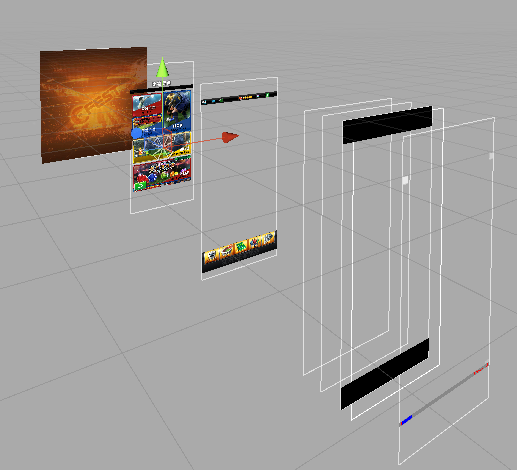
\includegraphics[scale=0.8]{CanvasFrame.png}
			\caption{Canvas 图层结构}
		\end{figure}
		
	在本项目中的所有画布的\textbf{渲染模式}均为 \verb|Screen-Camera| \textbf{模式}。
	
	\clearpage
	\subsection{图层结构组件}
		\dirtree{%
			.1 CvBack ->\textbf{背景层} .
				.2 画布参数 .
					.3 ->Camera: Main-Camera .
					.3 ->Distance: 800 .
					.3 ->Order: 0 .
				.2 BgEffectFest 背景特效.
				.2 BgBase .
					.3 MainHomeFestBgObj.
				.2 BgEffect .
				.2 BgWork .
		}
	
		\dirtree{%
			.1 Canvas ->\textbf{游戏层} .
				.2 画布参数 .
					.3 ->Camera: Main-Camera .
					.3 ->Distance: .
					.3 ->Order: .
				.2 Root .
				.2 MTHomeBaseObj .
				.2 MTHomeController .
				.2 MTHome.
				.2 MT\_01\_ScrollView .
		}
			
		\dirtree{%
			.1 CvMenu ->\textbf{目录层} .
				.2 画布参数 .
					.3 ->Camera: Mid-Camera .
					.3 ->Distance: 300 .
					.3 ->Order: 50 .
				.2 Empty .
					.3 HeaderRoot .
					.3 FooterRoot .
		}
	
		\dirtree{%
			.1 CvFade ->\textbf{渐退层} .
				.2 画布参数 .
					.3 ->Camera: Front-Camera .
					.3 ->Distance: 140 .
					.3 ->Order: 100 .
				.2 FadeImage .
		}
	
	\clearpage
		\dirtree{%
			.1 CvOverlap ->\textbf{交叠层} .
				.2 画布参数 .
					.3 ->Camera: Front-Camera .
					.3 ->Distance: 120 .
					.3 ->Order: 150 .
				.2 Empty .
				.2 CvOverlap2 ->交叠层2 .
					.3 画布参数 .
						.4 ->Camera: Front-Camera .
						.4 ->Distance: 90 .
						.4 ->Order: 180 .
		}
		
		\dirtree{%	
			.1 CvFore ->\textbf{黑框层} .
				.2 画布参数 .
					.3 ->Camera: Front-Camera .
					.3 ->Distance: 100 .
					.3 ->Order: 900 .
				.2 InputPanel .
					.3 top bottom Bg .
					.3 left rightBg .
				.2 NewSpinner .
				.2 DownloadingView .
		}
		
		\dirtree{%	
			.1 CvOverlapFull ->\textbf{网页层} .
				.2 画布参数 .
					.3 ->Camera: Front-Camera .
					.3 ->Distance: 90 .
					.3 ->Order: 180 .
				.2 WebViewTarget .
				.2 WebViewObject .
					.3 ImageBgTapArea .
					.3 ImageBg .
		}
		
		\dirtree{%	
			.1 CvDebug ->\textbf{调试层} .
				.2 画布参数 .
					.3 ->Camera: Front-Camera .
					.3 ->Distance: 50 .
					.3 ->Order: 999 .
				.2 DebugViewButton .
				.2 BackKeyButton .
				.2 DebugDispButton .
				.2 DebugPerfMeter .
		}


	\clearpage
	\subsection{图层渲染顺序说明}
		这个只针对在一个同一个相机下渲染的情况。在本项目中只针对\verb|Front-Camera|。渲染顺序如下所示:
			\begin{enumerate}
				\item CvFade 渐退层:100
				\item CvOverlap 覆盖层:150
				\item CvOverlap2 覆盖层2:180
				\item CvOverlapFull 网页层:180
				\item CvBug 调试层:999
			\end{enumerate}
		
		
\chapter{流程}
	\section{屏幕适配流程}
		\setlength{\DTbaselineskip}{20pt}
		\DTsetlength{1em}{3em}{0.1em}{1pt}{4pt}
		
		\paragraph{屏幕适配流程}
			\dirtree{%
				.1  .
				.2  \textbf{TitleBaseObj.cs}\\ .
				.2  判断是否为全面屏幕 ->isFullScreen = Screen.height / (float)Screen.width >= 1.95f; 首先判断屏幕高宽比例是否大于预设值,如果是便开启全面屏适配。 .
				.2  判断是否为非IPhone X 的全面屏幕 ->enableExpand = !IphoneXAdapt.IsBangPhone and isFullScreen; .
					.3  \textbf{IphoneXAdapt.cs  static函数}\\ .
				.2  如果是非IPhone X的全面屏幕.
					.3  \textbf{CanvasSetupManager.cs static函数}\\ .
					.3  ws.CanvasSetupManager.SetExpand(state) ->是否将“画布”设置为“展开”设置 .
					.4  if(expand != state) expand = state ->(true) .
					.4  modelAdapt() -> 机型适配.
						.5  vivo-X21 .
						.5  EML-AL00\&\&EML-TL100 .
						.5  CLT-AL00\&\&CLT-TL00\&\textbf{CLT-AL01} .
						.5  COR-AL00 .
						.5  其他 .
					.4  AllCanvasSetup() -> 共有 Canvas 调整.
					.4  cvMenu -> 页眉页脚调整.
					.4  SceneCanvasSetup() -> 画布调整当前场景.
			 }

		\clearpage
		\paragraph{TopOffset、BottomOffset 被使用函数}
			\dirtree{%
				.1  .
				.2 DTTopController.cs .
					.3 Start() ->目录列表TOP场景管理类 .
				.2 SupporterMainBaseObj.cs .
					.3 init(GameObject prefabSupport) ->初始化处理 .
				.2 SPMatchBaseObj.cs.
					.3 init() ->初始化处理 .
				.2 MatchSceneStartObj.cs .
					.3 IEnumerator SetUpLwf() ->LWF设置 .	
				.2 MTHomeBaseObj.cs ->游戏列表管理.
					.3 void Init() ->初始化处理-比赛界面打开优化 .
				.2 CanvasSetupManager.cs .
					.3 modelAdapt() ->机型适配->设置SET TopOffset、BottomOffset .
					.3 HeaderSetup() ->调整菜单页眉->GET TopBottom offset 进行页面调整 .
					.3 FooterSetup() ->调整菜单页脚->GET TopBottom offset 进行页面调整 .
					.3 setupRootObject() ->RootObject的RectTransform调整->GET TopBottom offset 进行页面调整 .
					.3 getTopHeight() ->获取上黑色区域高度->GET TopBottom offset 进行页面调整 .
					.3 getBottomHeight() ->获取下黑色区域高度->GET TopBottom offset 进行页面调整 .
					.3 AdjustAdapt() ->BaseObj适配(含header,footer)->GET TopBottom offset 进行页面调整 .
				.2 HeaderRoot.cs .
					.3 Start() .
			}	
			
		
		\clearpage
		\paragraph{modelAdapt() 具体流程细节}
			\dirtree{%
				.1  .
				.2 model = SystemInfo.deviceModel ->获取运行机型号 .
				.2 if(model.Contains("指定型号关键字")) ->判断是否为需要特殊处理的机型 .
				.3 TopOffset = \#define const ->设定顶端距离 .
				.3 BottomOffset = \#define const ->设定底部距离 .
				.3 openAdaptFlag = true ->刘海标记 .	
				.2 else .
				.3 TopOffset = 0 .
				.3 BottomOffset = 0 .
				.3 openAdaptFlag = false .
			}
		
		
		\paragraph{HeaderSetup(canvas, obj1) 具体流程细节}
			\dirtree{%
				.1 .
				.2 if (GetExpand ()) ->是否将“画布”设置为“expand”设置 .
					.3 target = targetSetup(target, obj2); ->在目标对象target上获取obj2对象,没有创建并将target 设置为其父节点,并返回 .
				.2 objectSetParent (target, obj); ->将target 设置为obj1 的父节点  .
				.2 addFooterImage () -> 添加页脚背景 .
				.2 obj.GetComponent<RectTransform> ().offsetMin = new Vector2 (0.0f, 0.0f - BottomOffset); -> 重新设置组件的矩形大小与位置 .		
			}
	
		%\paragraph{FooterSetup()}
	
	
		\paragraph{getTopHeight()}
			\dirtree{%
				.1 .
				.2 rate = Screen.width / 720.0f  .
				.2 height = Screen.height / rate .
				.2 if (height > 1280) .
				.3  height = GetExpand() ? (height - 1280)/2*rate-BottomOffset*rate : 0 .
				.2 else .
				.3 height = 0 .
			}
	
		%\paragraph{getBottomHeight()}
		
		
		\paragraph{AdjustAdapt(GameObject go)}
			\dirtree{%
				.1 .
				.2 if(go != null) .
				.3 设置Header RectTransform 位置 ->go.transform.Find("Header")\\ .GetComponent<RectTransform>().offsetMax .
				.3 设置Footer RectTransform 位置 ->go.transform.Find("Footer")\\ .GetComponent<RectTransform>().offsetMax . 
			}
		
		\paragraph{RootObject RectTransform 转换}
			\dirtree{%
				.1 setupRootObject(GameObject obj).
				.2 if(obj != null) .
				.3 if( GetExpand() ) ->非IPhone X全面屏幕 .
				.4 设置 RectTransform 位置 .
				.4 设置 锚点位置 .
				.3 else .
				.4 设置普通 RectTransform 位置 .
				.4 设置普通 锚点位置 . 
			}
		
		\paragraph{去掉黑色填补区域,并使用背景填充}\verb|->|
		
			适配刘海屏一般\textbf{上方区域不需要黑色填补区域},所以我们\textbf{关掉在刘海屏中上方黑色填补区域}。然后\textbf{把背景图进行同黑色填补区域长度的拉升}。
			
			(这里有个坑:黑色填补区域跟\verb|HeadRoot|\textbf{不在同一个}\verb|Canvas|,所以长度比例不一样,要进行转换,转换系数为:\verb|720f / Screen.width|)
			
			\dirtree{%
				.1 HeaderRoot.cs->Start() .
				.2 isFullScree ? .
				.2 enableExpand ? .
				.2 if(enableExpand \& openAdaptFlag) ->非iPhoneX的全面屏,并且刘海 .
				.3 设置区域 .
			}
			
		\paragraph{其他场景预制拉伸 -比赛界面}\verb|->|
		
			其他场景预制拉伸,并未测试所有场景
			
			比赛场景界面的ScrollView拉升。
			
			(这边也有个坑:之前的向上拉伸都是加上TopOffset,而现在却变成了(TopOffset+BottomOffset)/2,原因是:为了适配上下不同的程度的拉伸,我们进行了根节点的偏移,为了保证游戏中心点的准确。Root偏移之后上下拉升量便相等了。所以预制的拉伸为(TopOffset+BottomOffset)/2)
			
			\dirtree{%
				.1 MTHomeBaseObj.cs .
				.2 设置 scrollViewObj.GetComponent<RectTransform>().offsetMax .
				.2 设置 scrollViewObj.GetComponent<RectTransform>().offsetMin .
				.2 设置 scrollViewObj.GetComponent<RectTransform>().sizeDelta .
			}
	
	
	\section{Web 适配流程}
				
	 
	\section{添加荣耀球员描述}
		\paragraph{流程}
			
		\paragraph{相关变量}
			\begin{itemize}
				\item \verb|msCard.isGlory|
				\item \verb|_panel.setActive(true);|
			\end{itemize}
			
			
	\section{重复球员显示标记}
		\paragraph{替补球员显示流程}
			\dirtree{%
				.1 .
				.2 点击其他球队 onClickDispReserve() .
				.3 setReserveCard() .
				.4 \textbf{loadReserveCardImages()} .
				.5 loadCardImage() .	
			}
		
		\paragraph{在场球员显示流程}
			\dirtree{%
				.1 .
				.2 点击球队管理 .
				.3 \textbf{loadDeckCardImages()} .
				.4 loadCardImage() .
			}
	   
	   \paragraph{相关变量}
	   		\begin{itemize}
	   			\item \verb|FormationDataManager._dicAllDeckCardView[_Deck_Key]| 代表某球队(\verb|_Deck_Key|)的所有成员
	   			\item \verb|FormationDataManager._dicAllDeckCardView[_Deck_Key][0~17] | 代表某球队的某个球员
	   			\item \verb|_deckNow_AllUser.Add((LocalCardData.LocalCardData.localCardData[UserCardId]).CardId);| 将18名在场球员对应的角色卡片ID存入哈希表中
	   		\end{itemize}
   		
   			在\verb|loadReserveCardImages() |中,
   				\begin{lstlisting}[frame = L, xleftmargin = .079\textwidth]
   	FormationMainCardInfo[] objCards = FormationDataManager._objReserveCardTop.gameObject.GetComponentsInChildren<FormationMainCardInfo>();
   				\end{lstlisting}
   				
   			用于表示剩余球员的部分。
   			
   			在\verb|loadDeckCardImages() |中,
   				\begin{lstlisting}[frame = L, xleftmargin = .079\textwidth]
   	var temp = FormationDataManager._dicAllDeckUserCardIds[tempKey];
   	cnt = 0;
   	foreach (var temp2 in temp)
   	{
   		// 某个甲板(tempKey)场上的18名球员(temp2)
   	}
   				\end{lstlisting}
   			具体的球员表示如上,而卡片的具体表示如\textbf{相关变量}中的第3条(LocalData.localData..)。
   	
   	\section{福利活动未领取显示底部}
   		1- 在任务界面中,将\textbf{未领取}的福利显示\textbf{未完成}, 将领取的\textbf{放到界面底部}。
 		
 		2- 存在部分\textbf{可以多次领取}的奖励\textbf{在领取一次后不能再次领取}的bug
 		
 		\paragraph{界面结构}
 			\dirtree{%
 				.1 Welfare .
 				.2 WelfareController/BasePlate .
 				.3 Body/TabPlateRoot .
 				.4 ChargeRebatObj(Clone) .
 				.5 /Root/Content/ScrollView/ViewPort/Content.
 				.6 CommonPlateItemObj(Clone) .
 			}
 			
 			福利横条框集合
 			\verb|Content ->Scrow_View -> Vertical Layout Group|
 			
 			福利横条框
 			\verb|CommonPlateItemObj(Clone) -> CommonPlateItemObj.prefab| 
 			
 			福利条框核心组件
 			\begin{itemize}
 				\item \verb|desc1 |描述1
 				\item \verb|desc2 |描述2 
 				\item \verb|other |奖励
 				\item \verb|Button |领取按钮,修改部分
 				\item \verb|desc3 |描述3 (1/3)
 			\end{itemize}
 		
 		\paragraph{领取福利流程}
 			\dirtree{%
 				.1 .
 				.2 点击领取按钮 .
 				.3 CommonPlateItemObj.cs -> OnClickGetReward() .
 				.4 -> getRewardProc() .
 				.5 -> PushRedUpdate() .
 			}
 		
 		\paragraph{界面更新流程}
 			\dirtree{%
 				.1 .
 				.2 Scroll\_View -> Vertical Layout Group .
 				.3 ChargeRebatObj.cs ->RefreshView() .
 				.4 改变添加组件顺序即可 .
 			}
 		
 		\paragraph{领取福利显示不完全相关变量}
 			\begin{itemize}
 				\item Mission.isDone = true;
 				\item missionID
 				\item payMisFlags[missionId].Flag
 				\item misFlag = payMisFlags[missId].Flag == 1
 				\item Mission.isDone = misFlag.
 			\end{itemize}
 		
 		
 \chapter{相关技巧}
 	\section{黑框存在的合理性架构思考}
 	
 	\section{SVN 冲突解决}
 		  			
\end{document} 
 		    